\documentclass[border=125pt,tikz]{standalone}
\usetikzlibrary{arrows.meta,automata,positioning}

\begin{document}
    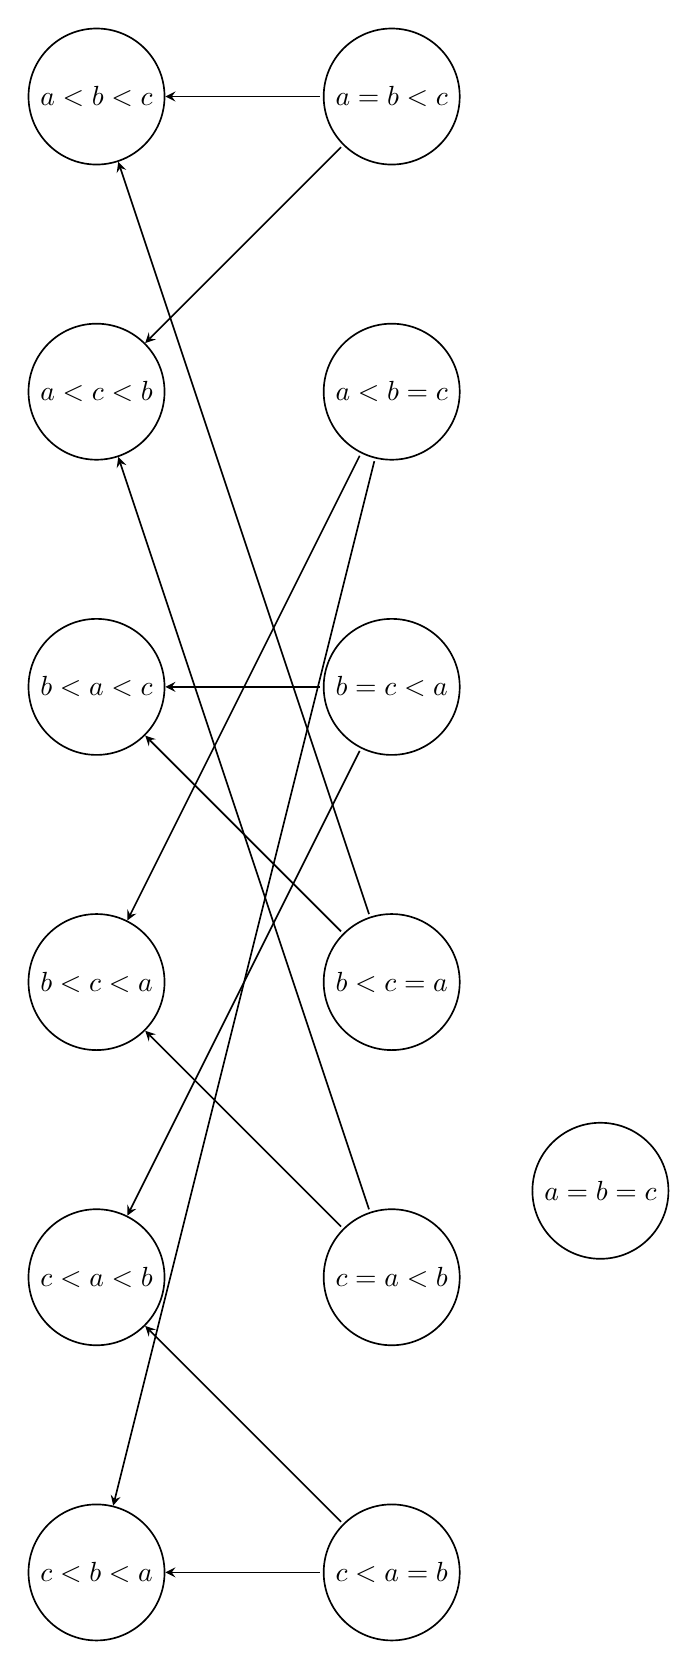
\begin{tikzpicture}[
    > = stealth, %
    shorten > = 1pt, %
    auto,
    node distance = 2cm, %
    semithick %
    ]

    \tikzset{every state}=[
    draw = black,
    thick,
    fill = gray,
    minimum size = 1mm
    ]

    \node[state] (x1)              {$a<b<c$};
    \node[state] (x2) [below=of x1]{$a<c<b$};
    \node[state] (x3) [below=of x2]{$b<a<c$};
    \node[state] (x4) [below=of x3]{$b<c<a$};
    \node[state] (x5) [below=of x4]{$c<a<b$};
    \node[state] (x6) [below=of x5]{$c<b<a$};

    \node[state] (y1) [right=of x1]{$a=b<c$};
    \node[state] (y2) [right=of x2]{$a<b=c$};
    \node[state] (y3) [right=of x3]{$b=c<a$};
    \node[state] (y4) [right=of x4]{$b<c=a$};
    \node[state] (y5) [right=of x5]{$c=a<b$};
    \node[state] (y6) [right=of x6]{$c<a=b$};

    \path[<-] (x1) edge  (y1);
    \path[<-] (x1) edge  (y4);
    \path[<-] (x2) edge  (y1);
    \path[<-] (x2) edge  (y5);
    \path[<-] (x3) edge  (y3);
    \path[<-] (x3) edge  (y4);
    \path[<-] (x4) edge  (y2);
    \path[<-] (x4) edge  (y5);
    \path[<-] (x5) edge  (y3);
    \path[<-] (x5) edge  (y6);
    \path[<-] (x6) edge  (y6);
    \path[<-] (x6) edge  (y2);
    
    \node[state] (z1) [below right =of y4]{$a=b=c$};

    

    \end{tikzpicture}
\end{document} 
